\documentclass{article}

% Language setting
% Replace `english' with e.g. `spanish' to change the document language
\usepackage[english]{babel}

% Set page size and margins
% Replace `letterpaper' with `a4paper' for UK/EU standard size
\usepackage[letterpaper,top=2cm,bottom=2cm,left=3cm,right=3cm,marginparwidth=1.75cm]{geometry}

% Useful packages
\usepackage{amsmath}
\usepackage{graphicx}
\usepackage[colorlinks=true, allcolors=blue]{hyperref}
\usepackage{amssymb}
\usepackage{tikz}
\usetikzlibrary{positioning, arrows.meta, quotes}

\title{Linear Algebra}
\date{}

\begin{document}
\maketitle

\tableofcontents

\newpage
\section{Matrix}
Matrix $A \in \mathbb{R}^{m \times n}$ defines a Linear Transformation from Domain $\mathbb{R}^n$ to Codomain $\mathbb{R}^m$.
\newline
Matrix $A$ is composed of column vectors $\mathbf{a}_j$, each of which is the image of the $j$-th standard basis vector after applying the transformation $A$.
\[
    A
\]
Expanded form~\ref{eq:matrix}


\newpage
\section{Matrix Operation}

\subsection{Inner Product}
The \textbf{Inner Product} (Dot Product) of two vectors $\mathbf{a}, \mathbf{b} \in \mathbb{R}^n$ is a scalar:
\[
    \langle \mathbf{a}, \mathbf{b} \rangle = \mathbf{a}^T \mathbf{b} = \sum_{i=1}^n a_i b_i
\]
Expanded form~\ref{eq:innerprod}.

\subsection{Norm}
The Euclidean Norm or $L^2$-norm of a vector $\mathbf{x} \in \mathbb{R}^n$, denoted as $\|\mathbf{x}\|$ or $\|\mathbf{x}\|_2$, is a measure of its Euclidean length.
\[
    \|\mathbf{x}\|^2 = \langle \mathbf{x}, \mathbf{x} \rangle = \mathbf{x}^T \mathbf{x}
\]

\subsection{Outer Product}
The \textbf{Outer Product} of two vectors $\mathbf{a} \in \mathbb{R}^m$ and $\mathbf{b} \in \mathbb{R}^n$ is an $m \times n$ matrix:
\[
    \mathbf{a} \otimes \mathbf{b} = \mathbf{a} \mathbf{b}^T
\]
Expanded form~\ref{eq:outerprod}.

\subsection{Matrix and Vector Multiplication}

\subsubsection{Matrix and Column Vector Multiplication}
Apply Linear Transformation $A \in \mathbb{R}^{m \times n}$ to vector $\mathbf{x} \in \mathbb{R}^n$ and produce a new vector $A\mathbf{x} \in \mathbb{R}^m$.
\[
    A\mathbf{x} = \sum_{j=1}^n x_j \mathbf{a}_j
\]
Expanded form~\ref{eq:matvec}.
\newline
\textbf{Geometric Interpretation:} Map the standard basis vectors in the Domain $\mathbb{R}^n$ to the column vectors in the Codomain $\mathbb{R}^m$.

\subsubsection{Row Vector and Matrix Multiplication}
Apply Linear Transformation $A \in \mathbb{R}^{m \times n}$ to a row vector $\mathbf{y}^T \in \mathbb{R}^{1 \times m}$ from the left and produce a new row vector $\mathbf{y}^T A \in \mathbb{R}^{1 \times n}$.
\[
    \mathbf{y}^T A = \sum_{i=1}^m y_i \mathbf{a}_i^T
\]
Expanded form~\ref{eq:rowvecmat}.
\newline
\textbf{Geometric Interpretation:} Map the standard basis vectors in the Codomain $\mathbb{R}^m$ to the row vectors in the Domain $\mathbb{R}^n$.

\subsection{Matrix and Matrix Multiplication}
Apply transformation $B$, then apply transformation $A$.
\[
    (AB)_{*j} = A\mathbf{b}_j
\]
Expanded form~\ref{eq:mul}.
\newline
\textbf{Associative Law:}
\[
    (AB)C = A(BC)
\]

\subsection{Inverse}
Reverses the transformation of $A$
\[
    A A^{-1} = A^{-1} A = I_n
\]
\textbf{Inverse of a Product Rule:}
\[
    (AB)^{-1} = B^{-1}A^{-1}
\]
\textbf{Properties:}
\begin{itemize}
    \item A square matrix $A \in \mathbb{R}^{n \times n}$ is invertible iff it has full rank, i.e., $\operatorname{rank}(A) = n$.
\end{itemize}
Calculation~\ref{subsec:gauss}.

\subsection{Determinant}
The \textbf{determinant} of a square matrix $A \in \mathbb{R}^{n \times n}$ is denoted as $\det(A)$ or $|A|$.
\newline
\textbf{Geometric Interpretation:} The scaling factor of the transformation $A$.
\newline
\textbf{Properties:}
\begin{itemize}
    \item A square matrix $A \in \mathbb{R}^{n \times n}$ has Full Rank iff $\det(A) \neq 0$.
\end{itemize}
\newline
\textbf{Calculation:}
\begin{itemize}
    \item \textbf{$2 \times 2$ Matrix:} For $A = \begin{bmatrix} a & b \\ c & d \end{bmatrix}$, $\det(A) = ad - bc$
    \item \textbf{$n \times n$ Matrix:}~\ref{subsec:cofactor}.
\end{itemize}

\subsection{Transpose}
\[
    (A^T)_{ij} = a_{ji}
\]
\[
    \langle A\mathbf{x}, \mathbf{y} \rangle = \langle \mathbf{x}, A^T\mathbf{y} \rangle
\]
Expanded form~\ref{eq:trans}.
\newline
\textbf{Geometric Interpretation:} Preserves the scaling factors of $A$ but reverses the rotation/reflection directions of $A$ by swapping domain and codomain orientations.
\newline
\textbf{Transpose Distribution Rule:}
\[
    (AB)^T = B^T A^T
\]


\newpage
\section{Vecctor Spaces and Subspaces}

\subsection{Linear Independence}
A set of vectors $\{\mathbf{v}_i\}_{i=1}^n$ is \textbf{Linearly Independent} if the only solution to the equation:
\[
    \sum_{i=1}^{n} c_i \mathbf{v}_i = \mathbf{0}
\]
is the trivial solution, where all coefficients $c_i = 0$. Otherwise, the set is \textbf{Linearly Dependent}.
\newline
\textbf{Geometric Interpretation:} Each vector in the set adds a new dimension to the space spanned by the others

\subsection{Column Space}
The \textbf{Column Space} (or \textbf{Range}) of a matrix $A \in \mathbb{R}^{m \times n}$ is the subspace of Codomain $\mathbb{R}^m$ spanned by the columns of $A$:
\[
    \text{Col}(A) = \{ A\mathbf{x} : \mathbf{x} \in \mathbb{R}^n \}
\]
\textbf{Geometric Interpretation:} The subspace of the Codomain representing all directions that \textbf{can be reached} by the transformation $A$.

\subsection{Null Space}
The \textbf{Null Space} (or \textbf{Kernel}) of a matrix $A \in \mathbb{R}^{m \times n}$ is:
\[
    \ker(A) = \{ \mathbf{x} \in \mathbb{R}^n : A\mathbf{x} = \mathbf{0} \}
\]
\textbf{Geometric Interpretation:} The subspace of the Domain containing the component of any input vector that is \textbf{discarded} by $A$.

\subsection{Row Space}
The \textbf{Row Space} of a matrix $A \in \mathbb{R}^{m \times n}$ is the subspace of Domain $\mathbb{R}^n$ spanned by the rows of $A$:
\[
    \text{Row}(A) = \{ \mathbf{y}^T A : \mathbf{y} \in \mathbb{R}^m \}
\]
\[
    \text{Row}(A) = \text{Col}(A^T)
\]
\textbf{Geometric Interpretation:} The subspace of the Domain containing the component of any input vector that is \textbf{preserved and transformed} by $A$.

\subsection{Left Null Space}
The \textbf{Left Null Space} (or \textbf{Cokernel}) of a matrix $A \in \mathbb{R}^{m \times n}$ is:
\[
    \operatorname{coker}(A) = \{ \mathbf{x} \in \mathbb{R}^m : \mathbf{x}^T A = \mathbf{0}^T \}
\]
\[
    \operatorname{coker}(A) = \ker(A^T) = \{ \mathbf{y} \in \mathbb{R}^m : A^T \mathbf{y} = \mathbf{0} \}
\]
\textbf{Geometric Interpretation:} The subspace of the Codomain representing all directions that \textbf{cannot be reached} by the transformation $A$.

\subsection{Rank}
The \textbf{Rank} of a matrix $A$ is the dimension of the Column Space or Row Space of $A$.
\newline
\textbf{Codomain:}
\newline
The Column Space is the \textbf{orthogonal complement} of the Left Null Space: $\text{Col}(A) = (\operatorname{coker}(A))^{\perp}$
\[
    \operatorname{rank}(A) + \dim(\operatorname{coker}(A)) = m
\]
\textbf{Domain:}
\newline
The Row Space is the \textbf{orthogonal complement} of the Null Space: $\text{Row}(A) = (\ker(A))^{\perp}$
\[
    \operatorname{rank}(A) + \dim(\ker(A)) = n
\]


\newpage
\section{Special Matrix}

\subsection{Identity Matrix}
The diagonal entries are all 1, and all off-diagonal entries are 0.
\[
    (I_n)_{ij} =
    \begin{cases}
        1, & i = j \\
        0, & i \neq j
    \end{cases}
\]
Expanded form~\ref{eq:iden}.
\newline
\textbf{Geometric Interpretation:} No transformation

\subsection{Diagonal Matrix}
The diagonal entries can be any value, and all off-diagonal entries are 0.
\[
    (D_n)_{ij} =
    \begin{cases}
        d_i, & i = j \\
        0, & i \neq j
    \end{cases}
\]
Expanded form~\ref{eq:diagm}.
\newline
\textbf{Geometric Interpretation:} Scale the $i$-th standard basis vector by $d_i$
\newline
\textbf{Inverse of a Diagnal Matrix:}
\[
    (D_n^{-1})_{ij} =
    \begin{cases}
        \frac{1}{d_i}, & i = j \\
        0, & i \neq j
    \end{cases}
\]
Expanded form~\ref{eq:diagminv}.

\subsection{Orthogonal Matrix}
All column vectors are unit vectors and orthogonal to each other.
\[
    Q^T Q = Q Q^T = I_n
\]
\[
    Q^T = Q^{-1}
\]
\textbf{Geometric Interpretation:} Rotation or reflection

\subsection{Symmetric Matrix}
\[
    A = A^T
\]
\textbf{Geometric Interpretation:} Scaling Transformation along orthogonal basis.
\newline
\textbf{Properties:}
\begin{itemize}
    \item Eigenvectors corresponding to distinct eigenvalues are orthogonal.
\end{itemize}


\newpage
\section{Matrix Decomposision}

\subsection{Eigenvector \& Eigenvalue}

A unit \textbf{Eigenvector} $\|\mathbf{v}\| = 1$ of a matrix $A \in \mathbb{R}^{n \times n}$ is scaled by its corresponding \textbf{Eigenvalue} $\lambda$ when the transformation $A$ is applied.
\[
    A\mathbf{v} = \lambda \mathbf{v}
\]
Calculation:
\[
    \det(A - \lambda I) = 0
\]

\subsection{Spectral Decomposition}

Symmetric matrix $A \in \mathbb{R}^{n \times n}$ can be decomposed as:
\[
    A = Q \Lambda Q^T
\]
where:
\begin{itemize}
    \item $Q$ is an orthogonal matrix whose columns are a set of orthonormal Eigenvectors of $A$.
    \item $\Lambda$ is a diagonal matrix whose diagonal entries are the Eigenvalues of $A$.
\end{itemize}
\textbf{Geometric Interpretation:}
\begin{enumerate}
    \item $Q^T$: Rotate or reflect the basis of the vector space to the Eigenvector basis.
    \item $\Lambda$: Apply a scaling transformation along the new axes by the Eigenvalues.
    \item $Q$: Rotate or reflect the basis of the vector space back to the standard basis.
\end{enumerate}

\subsection{Positive Definite}
A symmetric matrix $A \in \mathbb{R}^{n \times n}$ is \textbf{positive definite}, denoted as $A \succ 0$, if for any nonzero vector $\mathbf{x} \in \mathbb{R}^n$,
\[
    \mathbf{x}^T A \mathbf{x} > 0
\]
\textbf{Properties:}
\begin{itemize}
    \item All Eigenvalues of $A$ are positive. (Proof via Spectral Decomposition)
    \item $A$ is invertible, and $A^{-1}$ is also positive definite.
\end{itemize}

\subsection{Positive Semi-Definite}
A symmetric matrix $A \in \mathbb{R}^{n \times n}$ is \textbf{positive semi-definite}, denoted as $A \succeq 0$, if for any vector $\mathbf{x} \in \mathbb{R}^n$,
\[
    \mathbf{x}^T A \mathbf{x} \geq 0
\]
\textbf{Properties:}
\begin{itemize}
    \item All Eigenvalues of $A$ are non-negative. (Proof via Spectral Decomposition)
\end{itemize}

\subsection{Eigen Decomposition}

Square matrix $A \in \mathbb{R}^{n \times n}$ can be decomposed as ($A$ is \textbf{similar} to $D$):
\[
    A = P \Lambda P ^{-1}
\]
where:
\begin{itemize}
    \item $P$ is a matrix whose columns are the Eigenvectors of $A$.
    \item $\Lambda$ is a diagonal matrix whose diagonal entries are the Eigenvalues of $A$.
\end{itemize}
\textbf{Geometric Interpretation:}
\begin{enumerate}
    \item $P^{-1}$: Change the basis of the vector space to the Eigenvector basis.
    \item $\Lambda$: Apply a scaling transformation along the new axes by the Eigenvalues.
    \item $P$: Change the basis of the vector space back to the standard basis.
\end{enumerate}

\subsection{Singular Value Decomposition}

\subsubsection{Singular Vector \& Singular Value}
For any matrix $A \in \mathbb{R}^{m \times n}$ with rank $r$:
\begin{itemize}
    \item \textbf{Singular Values:} $\sigma_1 \geq \cdots \geq \sigma_r > 0$ represent the scaling factors along the principal directions of the transformation.
    \item \textbf{Right Singular Vectors:} Orthonormal basis for the Domain subspaces:
        \begin{itemize}
            \item First $r$ columns of $V$: orthonormal basis for $\text{Row}(A)$
            \item Last $n-r$ columns of $V$: orthonormal basis for $\ker(A)$
        \end{itemize}
    \item \textbf{Left Singular Vectors} Orthonormal basis for the Codomain subspaces:
        \begin{itemize}
            \item First $r$ columns of $U$: orthonormal basis for $\text{Col}(A)$
            \item Last $m-r$ columns of $U$: orthonormal basis for $\operatorname{coker}(A)$
        \end{itemize}
\end{itemize}

\subsubsection{SVD Formula}
Any matrix $A \in \mathbb{R}^{m \times n}$ can be decomposed as:
\[
    A = U \Sigma V^T = \sum_{i=1}^{r} \sigma_i \mathbf{u}_i \mathbf{v}_i^T
\]
where:
\begin{itemize}
    \item $V \in \mathbb{R}^{n \times n}$ is an orthogonal matrix whose columns $\mathbf{v}_i$ are the \textbf{Right Singular Vectors} of $A$.
    \item $U \in \mathbb{R}^{m \times m}$ is an orthogonal matrix whose columns $\mathbf{u}_i$ are the \textbf{Left Singular Vectors} of $A$.
    \item $\Sigma \in \mathbb{R}^{m \times n}$ is a diagonal matrix whose diagonal entries $\sigma_i$ are the \textbf{Singular Values} of $A$.
    \item $r = \operatorname{rank}(A)$ is the number of non-zero singular values.
\end{itemize}
\newline
\textbf{Geometric Interpretation:}
\begin{enumerate}
    \item \textbf{$V^T$:} Rotate or reflect the Domain $\mathbb{R}^n$ from the standard basis to the principal directions defined by Right Singular Vectors:
    \begin{itemize}
        \item The first $r$ standard basis vectors align with the orthonormal basis of $\text{Row}(A)$
        \item The last $n-r$ standard basis vectors align with the orthonormal basis of $\ker(A)$
    \end{itemize}

    \item \textbf{$\Sigma$:} Scale along each principal axis defined by the Singular Vectors:
    \begin{itemize}
        \item Scale the first $r$ axes (corresponding to $\text{Row}(A)$) by singular values $\sigma_1, \ldots, \sigma_r$
        \item Scale the last $n-r$ axes (corresponding to $\ker(A)$) by zero
        \item Map the $\text{Row}(A)$ directions to the $\text{Col}(A)$ directions
    \end{itemize}

    \item \textbf{$U$:} Rotate or reflect the Codomain $\mathbb{R}^m$ from the principal directions defined by Left Singular Vectors to the standard basis:
    \begin{itemize}
        \item The orthonormal basis of $\text{Col}(A)$ aligns with the first $r$ standard basis vectors
        \item The orthonormal basis of $\operatorname{coker}(A)$ aligns with the last $m-r$ standard basis vectors
    \end{itemize}
\end{enumerate}

\subsubsection{SVD Derivation}
Assume that matrix $A \in \mathbb{R}^{m \times n}$ can be decomposed as:
\[
    A = U \Sigma V^T
\]
where $U \in \mathbb{R}^{m \times m}$ and $V \in \mathbb{R}^{n \times n}$ are orthogonal matrices, and $\Sigma \in \mathbb{R}^{m \times n}$ is a diagonal matrix.

\paragraph{Compute $A^T A$ and $AA^T$:}
\[
    A^T A = (U \Sigma V^T)^T (U \Sigma V^T) = V \Sigma^T U^T U \Sigma V^T = V \Sigma^T \Sigma V^T
\]
\[
    AA^T = (U \Sigma V^T)(U \Sigma V^T)^T = U \Sigma V^T V \Sigma^T U^T = U \Sigma \Sigma^T U^T
\]
Notice that these expressions are in the form of Spectral Decomposition:
\begin{itemize}
    \item $A^T A = V (\Sigma^T \Sigma) V^T$ where $V$ is orthogonal and $\Sigma^T \Sigma$ is diagonal
    \item $AA^T = U (\Sigma \Sigma^T) U^T$ where $U$ is orthogonal and $\Sigma \Sigma^T$ is diagonal
\end{itemize}
Therefore: $V$ contains the Eigenvectors of $A^T A$, and $\sigma_i = \sqrt{\lambda_i}$. $U$ contains the Eigenvectors of $AA^T$, and $\sigma_i = \sqrt{\lambda_i}$.


\newpage
\section{Pseudo Inverse and Normal Equations}

\subsection{Pseudo Inverse}

For any matrix $A \in \mathbb{R}^{m \times n}$ with SVD $A = U \Sigma V^T$, the \textbf{Moore-Penrose Pseudo Inverse} is:
\[
    A^+ = V \Sigma^+ U^T
\]
where $\Sigma^+ \in \mathbb{R}^{n \times m}$ is defined element-wise as:
\[
    (\Sigma^+)_{ij} =
    \begin{cases}
        \frac{1}{\sigma_j}, & \text{if } i = j \text{ and } \sigma_j \neq 0 \\
        0, & \text{otherwise}
    \end{cases}
\]

\subsection{Normal Equations}

Minimize $\|A\mathbf{x} - \mathbf{b}\|^2$ for linear system $A\mathbf{x} = \mathbf{b}$ where $A \in \mathbb{R}^{m \times n}$,
\[
    A^T A \mathbf{x} = A^T \mathbf{b}
\]
\textbf{Derivation:} To minimize $\|A\mathbf{x} - \mathbf{b}\|^2$, the residual $A\mathbf{x} - \mathbf{b}$ is orthogonal to the column space of $A$, i.e., it belongs to the left null space $\operatorname{coker}(A)$
\[
    A^T(A\mathbf{x} - \mathbf{b}) = \mathbf{0}
\]


\newpage
\section{Quadratic Form}

\subsection{Quadratic Form}
For a vector $\mathbf{x} \in \mathbb{R}^n$, a quadratic form is:
\[
    q(\mathbf{x}) = \mathbf{x}^T A \mathbf{x}
\]
where $A \in \mathbb{R}^{n \times n}$ is a symmetric matrix.

\subsection{Geometric Interpretation}
The quadratic form $q(\mathbf{x}) = \mathbf{x}^T A \mathbf{x}$ describes the geometry of a quadric surface.

\paragraph{Apply Spectral Decomposition:}
\[
    q(\mathbf{x}) = \mathbf{x}^T (Q \Lambda Q^T) \mathbf{x} = (\mathbf{x}^T Q) \Lambda (Q^T \mathbf{x})
\]
Define $\mathbf{y} = Q^T \mathbf{x}$:
\[
    q(\mathbf{y}) = \mathbf{y}^T \Lambda \mathbf{y} = \sum_{i=1}^n \lambda_i y_i^2
\]
\begin{enumerate}
    \item The \textbf{Eigenvectors} of $A$ (columns of $Q$) define the \textbf{principal axes} of the geometric shape.
    \item The \textbf{Eigenvalues} $\lambda_i$ of $A$ \textbf{scales} the length of each semi-axis by $1/\sqrt{\lambda_i}$.
\end{enumerate}


\newpage
\section{Calculation}

\subsection{Gaussian Elimination}
\label{subsec:gauss}

Gaussian elimination is an algorithm for solving systems of linear equations, finding the rank, and calculating the inverse of a matrix. The process consists of two main steps:

\begin{enumerate}
    \item \textbf{Forward Elimination:} Transform the matrix into an upper triangular form using \textbf{elementary row operations}:
    \begin{itemize}
        \item Swap two rows.
        \item Multiply a row by a nonzero scalar.
        \item Add a multiple of one row to another row.
    \end{itemize}
    \item \textbf{Back Substitution:} Solve for the variables starting from the last row and moving upwards.
\end{enumerate}

\subsection{Cofactor Expansion}
\label{subsec:cofactor}
The determinant of a matrix can be calculated using Cofactor Expansion (or Laplace Expansion) along any row or column. For matrix $A \in \mathbb{R}^{n \times n}$, the expansion along the $i$-th row is:
\[
    \det(A) = \sum_{j=1}^{n} (-1)^{i+j} a_{ij} M_{ij}
\]
where $M_{ij}$ is the determinant of the submatrix obtained by removing the $i$-th row and $j$-th column.


\newpage
\section{Conceptual Mind Map}

\begin{figure}[h!]
\centering
\resizebox{\textwidth}{!}{%
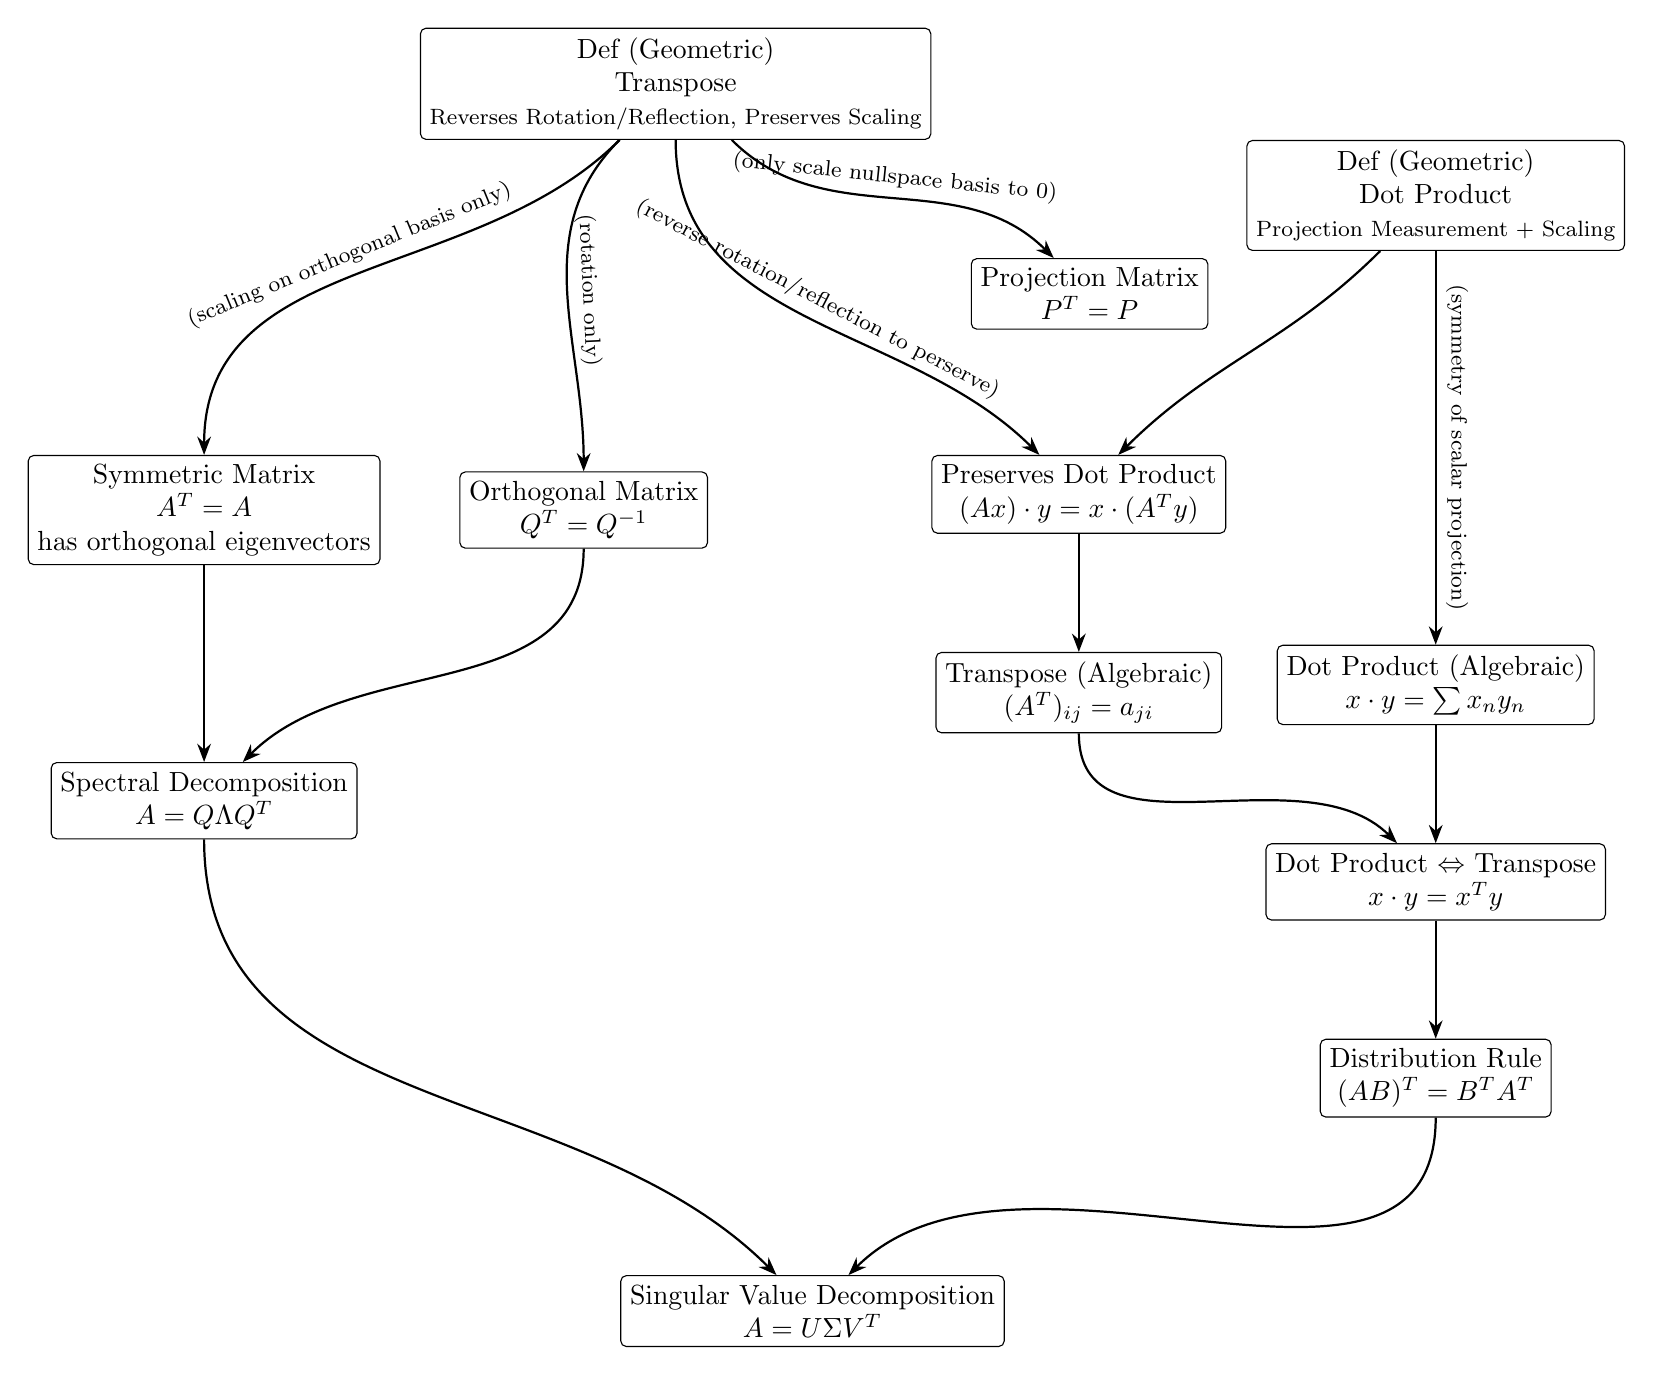
\begin{tikzpicture}[
    node distance=1.2cm and 1.5cm,
    concept/.style={align=center, draw, rounded corners=2pt},
    label/.style={sloped, font=\footnotesize, midway},
    arrow/.style={-Stealth, thick}
]
    % NODES
    \node[concept] (transpose_geo) {Def (Geometric) \\ Transpose \\ \footnotesize{Reverses Rotation/Reflection, Preserves Scaling}};
    \node[concept, below right=0cm and 4cm of transpose_geo] (dot_prod_geo) {Def (Geometric) \\ Dot Product \\ \footnotesize{Projection Measurement + Scaling}};

    \node[concept, below left=4cm and 0.5cm of transpose_geo] (symmetric) {Symmetric Matrix \\ $A^T=A$ \\ has orthogonal eigenvectors};
    \node[concept, right=1cm of symmetric] (orthogonal) {Orthogonal Matrix \\ $Q^T=Q^{-1}$};
    \node[concept, below right=4cm and 0cm of transpose_geo] (preserves_dot) {Preserves Dot Product \\ $(Ax) \cdot y = x \cdot (A^T y)$};
    \node[concept, below right=1.5cm and 0.5cm of transpose_geo] (projection) {Projection Matrix \\ $P^T=P$};

    \node[concept, below=2.5cm of symmetric] (spectral) {Spectral Decomposition \\ $A = Q \Lambda Q^T$};
    \node[concept, below=1.5cm of preserves_dot] (transpose_alg) {Transpose (Algebraic) \\ $(A^T)_{ij} = a_{ji}$};
    \node[concept, below=5cm of dot_prod_geo] (dot_prod_alg) {Dot Product (Algebraic) \\ $x \cdot y = \sum x_n y_n$};

    \node[concept, below=1.5cm of dot_prod_alg] (dot_prod_transpose) {Dot Product $\Leftrightarrow$ Transpose \\ $x \cdot y = x^T y$};
    \node[concept, below=1.5cm of dot_prod_transpose] (dist_rule) {Distribution Rule \\ $(AB)^T = B^T A^T$};
    \node[concept, below left=2cm and 4cm of dist_rule] (svd) {Singular Value Decomposition \\ $A = U \Sigma V^T$};

    % EDGES
    \draw[arrow] (transpose_geo) to[out=-135, in=90] node[label, above] {(scaling on orthogonal basis only)} (symmetric);
    \draw[arrow] (transpose_geo) to[out=-135, in=90] node[label, above] {(rotation only)} (orthogonal);
    \draw[arrow] (transpose_geo) to[out=-90, in=135] node[label, above] {(reverse rotation/reflection to perserve)} (preserves_dot);
    \draw[arrow] (transpose_geo) to[out=-45, in=135] node[label, above] {(only scale nullspace basis to 0)} (projection);

    \draw[arrow] (symmetric) to[out=-90, in=90] (spectral);
    \draw[arrow] (orthogonal) to[out=-90, in=45] (spectral);

    \draw[arrow] (dot_prod_geo) to[out=-90, in=90] node[label, above] {(symmetry of scalar projection)} (dot_prod_alg);
    \draw[arrow] (dot_prod_geo) to[out=-135, in=45] (preserves_dot);

    \draw[arrow] (preserves_dot) to[out=-90, in=90] (transpose_alg);
    \draw[arrow] (transpose_alg) to[out=-90, in=135] (dot_prod_transpose);
    \draw[arrow] (dot_prod_alg) to[out=-90, in=90] (dot_prod_transpose);

    \draw[arrow] (dot_prod_transpose) to[out=-90, in=90] (dist_rule);

    \draw[arrow] (spectral) to[out=-90, in=135] (svd);
    \draw[arrow] (dist_rule) to[out=-90, in=45] (svd);

\end{tikzpicture}
}
\end{figure}


\newpage
\appendix
\section{Expanded Form}

\begin{itemize}

    \item \textbf{Matrix:}
    \begin{equation}
        A =
        \left[
            \begin{array}{ccc}
                | &        & | \\
                \mathbf{a}_1 & \cdots & \mathbf{a}_n \\
                | &        & |
            \end{array}
        \right]
        \label{eq:matrix}
    \end{equation}

    \item \textbf{Inner Product:}
    \begin{equation}
        \mathbf{a}^T \mathbf{b} =
        \left[
            \begin{array}{ccc}
                a_1 & \cdots & a_n
            \end{array}
        \right]
        \left[
            \begin{array}{c}
                b_1 \\
                \vdots \\
                b_n
            \end{array}
        \right]
        = a_1 b_1 + \cdots + a_n b_n
        \label{eq:innerprod}
    \end{equation}

    \item \textbf{Outer Product:}
    \begin{equation}
        \mathbf{a} \mathbf{b}^T =
        \left[
            \begin{array}{c}
                a_1 \\
                \vdots \\
                a_m
            \end{array}
        \right]
        \left[
            \begin{array}{ccc}
                b_1 & \cdots & b_n
            \end{array}
        \right]
        =
        \left[
            \begin{array}{ccc}
                a_1 b_1 & \cdots & a_1 b_n \\
                \vdots & \ddots & \vdots \\
                a_m b_1 & \cdots & a_m b_n
            \end{array}
        \right]
        \label{eq:outerprod}
    \end{equation}

    \item \textbf{Matrix-Vector Multiplication:}
    \begin{equation}
        A\mathbf{x} =
        \left[
            \begin{array}{ccc}
                | &        & | \\
                \mathbf{a}_1 & \cdots & \mathbf{a}_n \\
                | &        & |
            \end{array}
        \right]
        \left[
            \begin{array}{c}
                x_1 \\
                \vdots \\
                x_n
            \end{array}
        \right]
        =
        x_1\mathbf{a}_1 + x_2\mathbf{a}_2 + \cdots + x_n\mathbf{a}_n
        \label{eq:matvec}
    \end{equation}

    \item \textbf{Row Vector-Matrix Multiplication:}
    \begin{equation}
        \mathbf{y}^T A =
        \left[
            \begin{array}{ccc}
                y_1 & \cdots & y_m
            \end{array}
        \right]
        \left[
            \begin{array}{c}
                - \mathbf{a}_1^T - \\
                \vdots \\
                - \mathbf{a}_m^T -
            \end{array}
        \right]
        =
        y_1\mathbf{a}_1^T + y_2\mathbf{a}_2^T + \cdots + y_m\mathbf{a}_m^T
        \label{eq:rowvecmat}
    \end{equation}

    \item \textbf{Matrix-Matrix Multiplication:}
    \begin{equation}
        AB =
        \left[
            \begin{array}{ccc}
                | &        & | \\
                A\mathbf{b}_1 & \cdots & A\mathbf{b}_p \\
                | &        & |
            \end{array}
        \right]
        \label{eq:mul}
    \end{equation}

    \item \textbf{Transpose:}
    \begin{equation}
        \left[
            \begin{array}{ccc}
                a_{11} & \cdots & a_{1n} \\
                \vdots & \ddots & \vdots \\
                a_{m1} & \cdots & a_{mn}
            \end{array}
        \right]^T
        =
        \left[
            \begin{array}{ccc}
                a_{11} & \cdots & a_{m1} \\
                \vdots & \ddots & \vdots \\
                a_{1n} & \cdots & a_{mn}
            \end{array}
        \right]
        \label{eq:trans}
    \end{equation}

    \item \textbf{Identity Matrix:}
    \begin{equation}
        I_n =
        \left[
            \begin{array}{cccc}
                1 & 0 & \cdots & 0 \\
                0 & 1 & \cdots & 0 \\
                \vdots & \vdots & \ddots & \vdots \\
                0 & 0 & \cdots & 1
            \end{array}
        \right]
        \label{eq:iden}
    \end{equation}

    \item \textbf{Diagonal Matrix:}
    \begin{equation}
        D_n =
        \left[
            \begin{array}{cccc}
                d_1 & 0 & \cdots & 0 \\
                0 & d_2 & \cdots & 0 \\
                \vdots & \vdots & \ddots & \vdots \\
                0 & 0 & \cdots & d_n
            \end{array}
        \right]
        \label{eq:diagm}
    \end{equation}

    \item \textbf{Inverse of Diagonal Matrix:}
    \begin{equation}
        D_n^{-1} =
        \left[
            \begin{array}{cccc}
                \frac{1}{d_1} & 0 & \cdots & 0 \\
                0 & \frac{1}{d_2} & \cdots & 0 \\
                \vdots & \vdots & \ddots & \vdots \\
                0 & 0 & \cdots & \frac{1}{d_n}
            \end{array}
        \right]
        \label{eq:diagminv}
    \end{equation}

\end{itemize}

\end{document}